% Generated by thesis/ch7/exp1/make_figures.py -- do not edit by hand.
\begin{figure}[tbp]
  \centering
  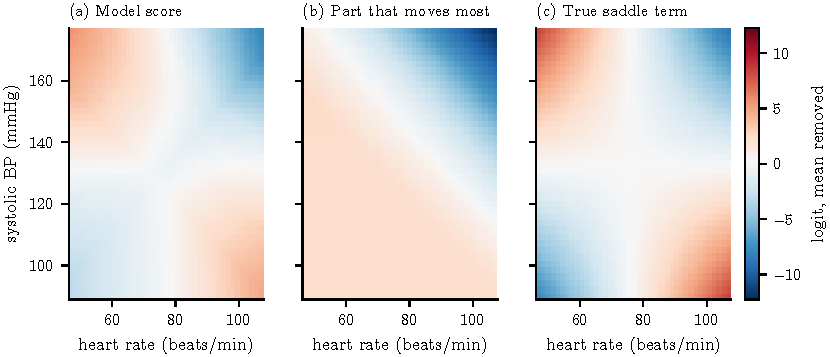
\includegraphics[width=\textwidth,height=0.8\textheight,keepaspectratio]{figures/ch7/options/synthetic-shape-b-saddle}
  \caption{Synthetic data (saddle only), the explained network: heart rate $\times$ systolic BP. Colour: the logit with its mean over the grid removed, one scale for all panels (red above the mean, blue below); every other input at the typical case. (b) The explanation part whose contribution moves most on the grid (\emph{pressure rate load}). True term: $-1.5\,z_h z_p$ (standardised heart rate and systolic BP).}
  \label{fig:ch7-synthetic-shape-b-saddle}
\end{figure}
